% -*-cap2.tex-*-
% Este fichero es parte de la plantilla LaTeX para
% la realización de Proyectos Final de Carrera, protegido
% bajo los términos de la licencia GFDL.
% Para más información, la licencia completa viene incluida en el
% fichero fdl-1.3.tex

% Copyright (C) 2009 Pablo Recio Quijano 

\section{El dominó}

\subsection{Historia del dominó}

El dominó, deporte y pasatiempo a un tiempo, es un juego que ha ganado adeptos a lo largo de la historia
y del tiempo. Según explica \textbf{Miguel Lugo} en su libro Dominó Competitivo \cite{lugo08} éste “es entretenido y fácil de
aprender. Ya desde pequeños comenzamos a jugar al dominó con frutas o con animales en lugar de hacerlo
con puntos”. Además, éste ha ganado popularidad durante los últimos años hasta el punto de televisar
torneos en Europa, Norteamérica y Latinoamérica.

\begin{quote}
“En 2001 la Federación Internacional de Dominó (con sede en Barcelona, España) celebró el primer
Congreso Internacional. El año siguiente se llevó a cabo el primer Campeonato del Mundo de Dominó en La
Habana (Cuba). El ‘Mundial’ continúa celebrándose anualmente a partir de este punto, en España, México,
Venezuela y EEUU" (Lugo, 2008: 1).
\end{quote}

Así pues Lugo señala que el dominó nunca antes ha estado tan reconocido en todo el mundo como ahora e
incluso afirma que se puede jugar por Internet. \\

La página web Dominó en Línea \cite{website:dominoenlinea} recoge que en la actualidad el dominó se juegan en todo el
mundo aunque resalta que es “especialmente popular en América Latina, donde los dominós se consideran
como el juego nacional de numerosos países del Caribe”. Así, también menciona los torneos anuales y
los clubes locales de dominó.

\begin{quote}
El origen del dominó parece ser muy antiguo, al menos en lo que se refiere a juegos similares y quizá
pretéritos al actual” (González Sanz, 2010:22)
\end{quote}

Cuenta \textbf{González Sanz} en su libro El arte del dominó: teoría y práctica \cite{sanz00} que algunos historiadores
creen que puede tener origen chino, ya que éstos jugaban a un juego parecido con impresiones en piedra,
y que pudo llegar a Europa a través de mercaderes y viajeros, entre los que se cita al célebre
Marco Polo, los cuales y fruto de los intercambios culturales de la época, trajeron el dominó a este
lado del mundo, más en concreto a la Península Itálica, primer lugar de Europa donde se ha datado la
práctica de este juego. \\

\textbf{Benito Ruipérez} \cite{mora90} también señala que se trata de un juego muy antiguo, de unos 400 años de historia,
aunque dice que se desconoce su origen y etimología (1990:7). Por otro lado, este autor comenta que
llego a Italia desde China en el siglo XVIII, sin embargo, relata que no está probado. “Versiones
coincidentes aseguran que el dominó entró en Europa a través de Italia (con lo que también se puede
atribuir su invención a los italianos, al menos el sistema de juego europeo)”, recoge Ruipérez. \\

Los italianos lo pusieron de moda introduciéndolo en España y Francia a mediados del siglo XVIII,
llegando más tarde a popularizarse de modo extraordinario. A finales del mismo siglo apareció en
Inglaterra, donde fue calificado de ‘juego infantil’, según Ruipérez “nada más lejos de la realidad”.
\textbf{Joseph Strutt} publicó un libro Deportes y Pasatiempos en 1801, en el que, entre otros disparates,
demostró un gran desconocimiento del juego. Así, escribió: “El dominó no tiene mayor interés que
el ponerlo en conocimiento de las personas mayores de este país” (Ruipérez, 1990:7). \\

Precisamente \textbf{Martin Gardner}, experto en juegos, explica que en la literatura occidental no hay
referencias a este juego hasta mediados del siglo XVIII, en que empezaron a jugarse en Italia y
Francia las primeras partidas. Desde ahí, el juego se extendió al resto del continente, y más tarde,
a Inglaterra y América. En Occidente, la colección normal de piezas de dominó ha consistido siempre
en 28 teselas o losetas formadas por dos cuadrados adyacentes, que contienen todos los posibles
pares de dígitos, de 0 hasta 6. \\

\begin{figure}[h]
  \label{Martin_Gardner}
  \begin{center}
    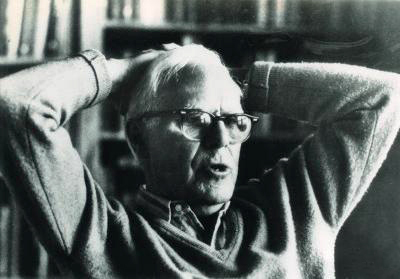
\includegraphics[scale=0.5]{Martin_Gardner.jpeg}
  \end{center}
  \caption{Martin Gardner, divulgador científico y filósofo de la ciencia estadounidense.}
\end{figure}


Respecto al juego chino, Gardner, que colaboró más de 20 años en la sección “Juegos Matemáticos” de
la revista \textbf{Scientific American}, comenta en su libro Circo Matemático que en los dominós chinos,
llamado kwat p’ai, no existen piezas con caras en blanco. Éstos contienen todas las combinaciones
por pares desde el (1-1)  hasta el (6-6), donde tres de los seis puntos de cara son también rojos.
Los dominós coreanos son idénticos, con la única particularidad de que en el as, el punto es mayor
que en las demás piezas. En los dominós chinos, cada pieza tiene un nombre pintoresco: el (6-6)
es el “cielo”; el (1-1) es “la tierra”, el (5-5) es la “flor del ciruelo”, el (6-5), “la cabeza de
tigre”, etc. Los nombres de las piezas son iguales a los que reciben los 21 resultados posibles del
lanzamiento de un par de dados. \\

Ruipérez añade que el invento se les achaca a los chinos “pero no ha de ser muy fiable, ya que el
dominó de chinos y coreanos es muy distinto al que se practica en Europa” (1990:7). Así lo describe
en su Libro del dominó:

\begin{quote}
“El dominó oriental consta de 21 fichas, que representan las permutaciones matemáticas resultantes
de tirar dos dados (cada mitad de una ficha vale por un lado), el ‘uno’ y el ‘cuatro’ son rojos;
además, en los dados chinos intervienen 11 fichas repetidas, con lo que suman un total de 32 fichas
el conjunto de, y para, este juego. Las fichas repetidas se llaman ‘civiles’ y las otras ‘militares’,
distinción importante para ciertos juegos de dominó en China y Corea”.
\end{quote}

González Sanz (2010:22) señala que los dominós chinos “suelen ser en la actualidad de cartón, en vez
de la madera, marfil, pasta, o ébano que es lo habitual en los occidentales, y se manejan como naipes”.
Y al igual que ocurre en Europa y América, con estas piezas se realizan numerosos juegos. Respecto a
los distintos juegos de dominó chinos y coreanos, este autor nos remite a Games of the Orient de Stewart
Culin, obra de 1895 reimpresa en 1958 por Charles Tuttle como la mejor referencia. Asimismo apunta que
no existe un dominó propio en Japón – frente al resto de países asiáticos – y dice que en este país se
juega con el sistema occidental. \\

\begin{figure}[h]
  \label{}
  \begin{center}
    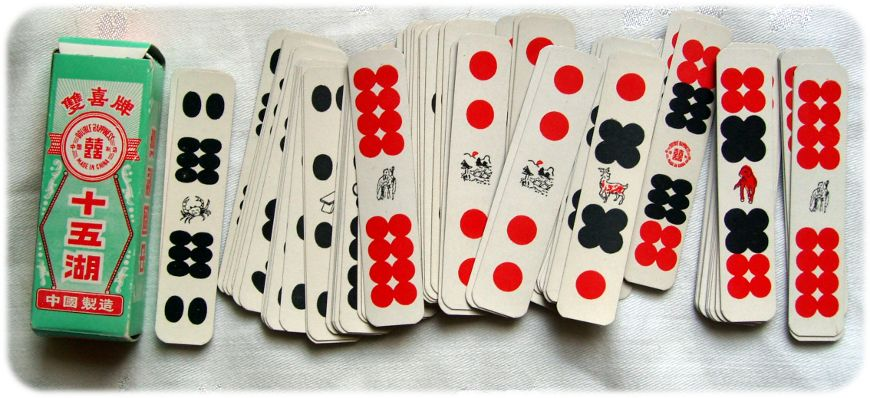
\includegraphics[scale=0.6]{chinese.jpg}
  \end{center}
  \caption{Cartas de dominó chino \textbf{“Double Happiness”} --- los símbolos representan diferentes
            circunstancias y bendiciones de la vida }
\end{figure}

Sin embargo, y aunque por lo que señalan algunos autores el origen asiático del dominó es el más
extendido, también existen otras versiones que atribuyen el invento del juego a árabes o egipcios,
“sosteniendo que no hay pruebas para relacionar claramente el dominó europeo con el chino, pudiendo
ser dos invenciones independientes y separadas en el tiempo” (2010:23). González también cuenta que
se conocen otras versiones del juego como la esquimal o la coreana, con distinto número de fichas
y palos al clásico. \\

Por otro lado, otros autores (desde la página Dominó en Línea \cite{website:dominoenlinea}) apuntan que el dominó
de origen más antiguo se habría encontrado en la tumba de Touthankamon en Egipto. \\

Los dominós nacieron de la derivación del juego de dados indio, conocido en Europa bajo el dado a
seis-cara, los chinos modificaron este dado en parte plana reversible representando puntos, de 1
en 6 puntos. En Europa sería apareció una cara suplementaria, el blanco. \\

En el apartado de curiosidades que se apunta en esta web podemos destacar que la palabra “dominó”
sería a causa de la semejanza entre las partes de las fichas del juego y la ropa de las religiosas
de las Dominicas (blanco cubierto de un cabo negro). Sin embargo, el autor Ruipérez en el Libro
del Dominó apunta otros posibles orígenes al término, algunos muy parecidos al ya apuntado. \\

En este sentido, señala este autor que su nombre se debe, según unos, al revestimiento negro que
llevan sus fichas por el reverso (la espalda), como si fueran cubiertas por un dominó (capuchón
que usaban en el coro, durante el invierno, los monjes). Y según otros, a que tal juego, por su
sencillez, “prueba inequívoca de que no se conocían las técnicas que se usan hoy en día, o de alta
escuela, que son las que se explican en este libro”, estuvo muy en uso en los conventos, y cuando
uno de los jugadores ganaba una partida decía: ‘Benedicamus Dómino’. Una tercera versión para
explicar el nombre afirma que por aquel entonces alguien ya detectó que para ‘manejar’ bien estas
fichas tenía que tener ‘dominio’ de sí mismo (control de lo jugado y de lo pendiente por jugar) en
cada mano, y podría decir, cada vez que querían jugar con estas fichas, ‘vamos a practicar unas
manos al juego del dominio’, habiendo degenerado o perfeccionado el dicho hasta quedar en el juego
del dominó (Ruipérez, 1990:9). \\

En cuanto a la documentación escrita de este juego, este mismo autor, Ruipérez, señala que el primer
libro que hace referencia al juego del dominó data del año 1786, editado en Amsterdam, según consta
en la Biblioteca Nacional de Bruselas. En total, este autor señala que hay más de un centenar de
libros hasta la fecha (1984), según consta también en distintas bibliotecas nacionales de Europa y
Latinoamérica. Aunque para este autor no han tenido suficiente éxito porque no se profundiza en
el tema sino que se relatan someramente las reglas básicas del mismo. \\

En 1982 y después en 1984, más reformado y actualizado, aparece en Barcelona el libro \textbf{ABC del dominó},
de J.M. Vilabella, que denota un conocimiento más amplio del tema comparado con lo que se había
escrito hasta ese momento, dando explicaciones más amplias de cómo se desarrollan las jugadas,
“aunque muy pocas y con muy pocas variantes”, (Ruipérez, 1990:8)

\subsubsection{Tipología de dominós}

Como hemos visto, a lo largo y ancho del mundo existen diferentes tipos de dominó de los que no
siempre los autores coinciden con un solo origen. Aunque para catalogar tales juegos como dominó sí
deben tener una serie de características en común. 

\begin{quote}
Generalizando el concepto de dominó, podríamos decir que es un juego cuyas fichas se encuentran
divididas en dos partes, las cuales señalan mediante incisiones o muescas, un número concreto entre
los posibles palos o números admitidos. Estas fichas contendrán en su totalidad todas las
combinaciones posibles de estos palos, comenzando por la ausencia de puntos o palo de blancos
(González Sanz, 2010:24).
\end{quote}

La Real Academia de la Lengua Española en su primera acepción define este juego como aquel que
“se hace con 28 fichas rectangulares divididas en dos cuadrados, cada uno de los cuales lleva marcados
de uno a seis puntos, o no lleva ninguno. Cada jugador pone por turno una ficha que tenga número
igual en uno de sus cuadrados al de cualquiera de los dos que están en los extremos de la línea de
las ya jugadas, y gana quien primero coloca todas las suyas o quien se quede con menos puntos, si
se cierra el juego”. De este modo, la RAE acota algo más el término acercándose a lo que conocemos
como dominó occidental. \\

Según la página Dominó en Línea \cite{website:dominoenlinea} “los dominós son de simples bloques de construcción
que pueden armarse de innombrables maneras con el fin de crear una gran variedad de juegos. Es un
juego que exige mucha capacidad y de estrategia”. \\

\begin{figure}[h]
  \label{Dominoes}
  \begin{center}
    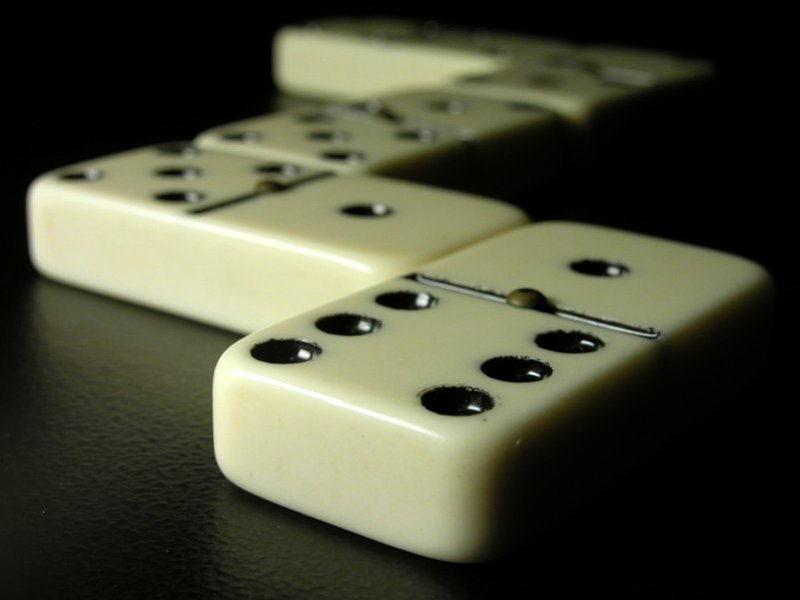
\includegraphics[scale=0.3]{Dominoes.jpg}
  \end{center}
  \caption{Fichas de dominó europeo}
\end{figure}


Ruipérez define el domino europeo en “un conjunto de veintiocho fichas, por lo general negras y
totalmente lisas por un lado, el reverso o la espalda, y por el otro lado, el anverso o la cara,
divididas en dos mitades con fondo blanco y señaladas con agujeros o puntitos negros; en el centro
de la cara llevan un tornillito con cabeza redondeada, que es el que apoya en la mesa y facilita
el movimiento de las fichas cuando éstas han de ser movidas (barajadas), para que los participantes
cojan sus fichas e inicien la jugada o la mano correspondiente. Tiene siete fichas denominadas
dobles, por en sus medias partes de la cara la misma cantidad de puntitos, a excepción de la
doble blanca, que no lleva ninguno”.

\subsection{Reglas básicas}
\subsection{Estructura de una partida simple}
\subsection{El dominó es un juego de señores}
\subsection{Juego por parejas}
\subsection{Técnicas avanzadas}

\section{Inteligencia artificial}

A la hora de afrontar un proyecto que simule cierto comportamiento \emph{humano}, debemos acercarnos a esa rama de la
Informática llamada Inteligencia Artificial, en busca de herramientas, técnicas y metodologías que nos ayuden a afrontar este
difícil problema, probablemente uno de los más complicados dentro de la Ingeniería Informática

\subsection{Sistemas expertos}

Para impregnar de inteligencia a los contrincantes de Dominous se utilizará lo que se suele llamar un \textbf{sistema experto}~\cite{Giarratano:1989:ESP:583478}.
Los sistemas expertos son una rama de la Inteligencia Artificial, que se basa en imitar los mecanismos y la forma de
pensar de un experto en cierta materia para resolver problemas de distinta índole.\\

Un Sistema Experto está conformado por:
\begin{description}
    \item[Base de conocimientos] Contiene conocimiento modelado extraído del diálogo con un experto.
    \item[Base de hechos (Memoria de trabajo)] Contiene los hechos sobre un problema que se ha descubierto durante el análisis.
    \item[Motor de inferencia] Modela el proceso de razonamiento humano.
    \item[Módulos de justificación] Explica el razonamiento utilizado por el sistema para llegar a una determinada conclusión.
    \item[Interfaz de usuario] Es la interacción entre el SE y el usuario, y se realiza mediante el lenguaje natural.
\end{description}

\subsection{Otros}
